\section{WhiteMesh Networks}
\label{sec:problemformulation}

In this section, we define and introduce WhiteMesh networks which jointly use WiFi and white space 
frequencies in a wireless mesh network. We then discuss the influences of WiFi and white 
space frequencies in wireless mesh network design. Further, we describe the two tiers we consider in 
wireless mesh network deployments: access and backhual tier.


\subsection{WhiteMesh Structure and Restrictions}
\label{subsec:problem}
% WhiteMesh concept
Here, the term WhiteMesh refers to a heterogeneous wireless network which jointly exploits 
both WiFi and white space frequencies. Thus, variation in frequency bands allows diverse 
capacity and service areas in network design.
% The Channel availability
% Available channel, propagation, 
The white space bands were originally assigned to analog TV broadcasting. The 
number of white space channels is typically less in dense areas than in the rural areas to protect the 
existing TV broadcasting networks. An example of available channels acroos a metropolitan area is shown in Fig.~\ref{fig:wschannels} (DFW). 
The diverse attributes at WiFi and white space bands impact network deployments in unique ways.
In sparse rural areas, the number of wired entry points to the Internet is like to be more restricted. 
At the same time, sparse populations generate relatively low amount of traffic 
demand. The lower traffic demand requires fewer spectral resources for users directly connecting access points
and may allocate more resources to links between access points (backhual tier).
Conversely, in densely-populated areas, there is likely a greater availability to wired entry points to the Internet.
At the same time, the dense population generates more traffic demand requiring greater use of spectral resources
for the access tier, leading to less using available for the backhual tier. 
As shown in Fig.~\ref{fig:wschannels}, the spectral resources in dense areas 
are also less available than in the sparse area. 
When there are more spectral resources reserved 
for the access tier, few spectral resources can be used for the backhual tier.


% Two extreme cases
Moreover, white space frequencies have longer wavelengths than WiFi frequencies. 
% Propagation
The strength of the received signal depends on both the line-of-sight path (or lack 
thereof) and multiple other paths that result from reflection, diffraction, and scattering 
from obstacles~\cite{andersen1995propagation}. The widely-used Friis equation characterizes 
the received signal power $P_r$ in terms of transmit power $P_t$, transmitter gain $G_t$, 
receiver gain $G_r$, wavelength $\lambda$ of the carrier frequency, distance $R$ from transmitter 
to receiver, and path loss exponent $n$ according to~\cite{friis}:
\begin{equation}
\label{eq:friis}
P_r=P_t+G_t+G_r+10n \log_{10}\left( \frac{\lambda}{4\pi R}\right)
\end{equation}
where, $n$ varies according to the aforementioned environmental factors with a value 
ranging from two to five in typical outdoor settings~\cite{rappaport}.
% Extreme cases
Thus, the propagation range of white space frequencies is longer than WiFi frequencies
given a similar environment. For the same transmit power, greater propagation levels leads to larger service area.
This effect could be beneficial for sparse areas since the traffic demand from the sparse population is relatively lower. 

The network deployment is constrained by the coverage area of a single access point. 
The large propagation regions of white spaces help to greatly reduce the number of access points and corresponding network cost. 
Conversely, a densely-populated area could saturate the capacity of a single white space channel. 
However, WiFi has smaller interference range and propagation range. The smaller interference range increases 
the spatial reuse of WiFi bands. In a densely-populated area, the network deployment is constrained by the 
capacity of a single access point. It is straightforward to solve the band selection problem in network deployment 
of these two extreme cases: (i) in a highly-sparse area, white space bands are better at aggregating the 
relatively lower traffic demand in larger areas; (ii) in a highly-dense area, WiFi bands are better 
for spatial reuse and these ally regions are less of available white spaces.
% Motivation of the work
However, the deployment is generally somewhere between these two extremes. 
To quantify and maximize the benefit of jointly using these bands, 
our work focuses on access and backhual design of WhiteMesh networks across varying population densities. 



\begin{figure}
\vspace{-0.0in}
\centering
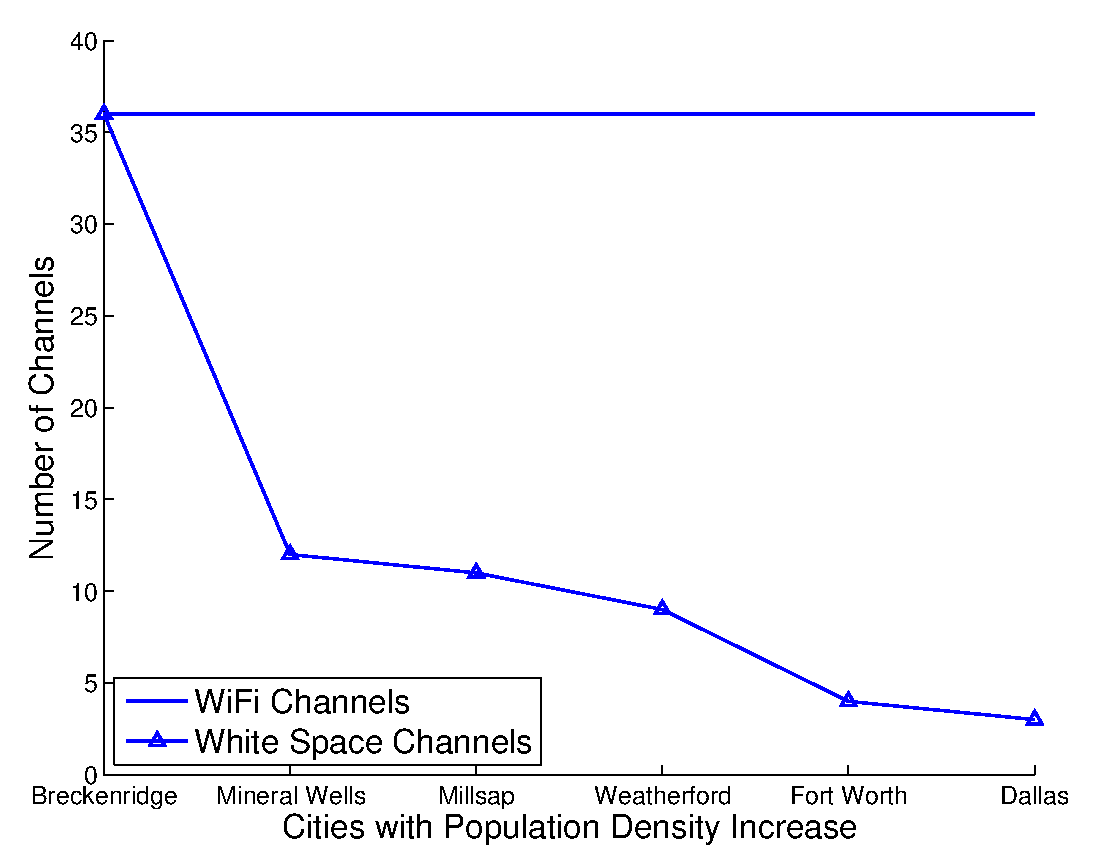
\includegraphics[width=64mm]{figures/wschannels}
\vspace{-0.1in}
\caption{WiFi and White Space Channels in North Texas}
\label{fig:wschannels}
\vspace{-0.3in}
\end{figure}


% The second part of wireless network deployment
\subsection{Wireless Mesh Network Deployment} 
% Network deployment objective

% Here Resource allocation





Wireless mesh networks have multihop paths between access points to reduce the number of wired entry points 
to the Internet and reduce network costs. 
The key objective of wireless network deployment is 
to serve the traffic demand of the population at a minimal financial cost, thereby increasing the long-term 
usability of the network. 
Many wireless networks have been implemented 
in school campuses, office buildings, and even mobile scenarios. Typically, wireless mesh networks 
have at least two tiers~\cite{CRSK06}: {\it (i)} an access tier, where users directly communicate to 
access points, and {\it (ii)} a multihop backhual tier for connecting all access points to the 
Internet through gateway nodes. 
% Network tiers
%Access tier serves user traffic demand which is often proportional to the population distribution in the 
%long term. The backhual tier iprovides Internet connectivity to the access tier. Naturally, the 
%capacity of wireless channels are limited which bring the trade off between the {\it Capacity} 
%and {\it Coverage}. Moreover, in wireless network design, another trade off between the 
%limited budget and the quality of service. To satisfy more people, a network requires more access points 
%in the access tier and more capacity in the backhual tier which ask for more budget. These are the 
%basic natural and artificial factors in network design.

\textbf{Access Tier.} 
% Network Constraint
An access point should ideally provide network capacity equal to the demand of the service 
area. The deployment of the access tier is subject to the coverage constraint of a given area and the capacity 
constraint of the users in the area. The coverage constraint is defined with respect to the ability of 
users to connect to access points within their service area. The capacity constraint is defined with 
respect to the ability of a network to serve the traffic demand of users. Spatial reuse allows improved 
capacity but increases the cost of deploying a large-scale network by increasing the total number of access points 
required. 

\textbf{Backhual Tier.} 
Access points may communicate directly to one another to form a backhual tier which forwards traffic to and from 
gateway points to reach the wired or wireless Internet entry points. 
%A backhual network without costly wires is provides more capacity to access tier. backhual network is 
%highly related to infrastructure. The infrastructure limits the available locations of backhual nodes. 
%That is the value of wireless backhual other than wired connection.
%Few flexilibility of backhual network allocation makes the assignment of the spectrum resource is a key 
%technology in backhual network design. 
Prior work focused on improving the capacity 
by reducing the interference among the links~\cite{si2010overview,doraghinejad2014channel}. 
%To improve the performance of citywide wireless network, we have to solve the issues in both access tier 
%and backhual tier. Lacking of consideration of either tier will result in a bottle neck for wireless 
%network design.
% Previous work focus on multichannel
% System model
However, many of these works assume a uniform propagation ability of the multiple channels used in the deployment.~\cite{doraghinejad2014channel}. 
In this work, we study the wireless network deployment across WiFi and white space frequencies, which have diverse 
propagation and availability based on the deployment location.
%For the access tier, 
%we focus on reducing the number of access points under the capacity and coverage constraints 
%jointly consider the propagation and utilization variations.
%For the backhual tier. to distinguish the dynamics of white space bands, we employ the activity
%level to represent the achieved channel capacity. 





 







% Metrics
%A wireless network is designed to satisfy the traffic demand from the users. Wireless networks are 
%operated and maintained by vendors, such as AT\&T, T-Mobile, who charge the customers based on their 
%data through Internet. In practice, the traffic demand of the user obey Poisson distribution~\cite{saaty1961elements}, 
%The satisfied traffic demand of the ursers are noted as served traffic flow. 
%The served traffic flow $X$, is represented as the traffic arrived at the gateway nodes to the 
%Internet in Eq.~\ref{eq:goodput}:
%\begin{equation}
%\label{eq:goodput}
%X=\sum_{w \in W, v \in V}T(w,v)
%\end{equation}
%The traffic arrived gateway node $w\in W$ includes all incoming and outgoing wireless traffic 
%from access node $v\in V$ as $T$ onto the Internet. 
%
%
%
%% Discuss the white space band in access and backhual
%% Traffic demand calculation
%White mesh network also has to satisfy the coverage constraint and capacity constraint in the access tier. 
%The coverage constraint could be calculated from~\ref{eq:friis} model. Generally, a coverage of $95\%$ of 
%access tier is acceptable for wireless access networks~\cite{robinson2010deploying}. We represent the capacity 
%constraint quantification as follow. The demand of a service area could be calculated as the 
%summation of individual demands all over the service area $D_a=\sum\limits_{p\in P} D_p$. Since household demand 
%for the Internet has been previously characterized~\cite{rosston2011household}, $D_a$ could represent the 
%population distribution $f$ and service area $k$ as $D_a=\sum\limits_{f \in F,k \in K}\bar{D_p}*f*k$. The capacity 
%constraint could be represented with an access point set $M$ according to:
%\begin{equation}
%\label{eq:nlbound}
%\sum_{m \in M}\delta_r^m \ge \sum_{f \in F,k \in K}\bar{D_p}*f*k
%\end{equation}
%
%% Interference
%Interference is a key issue in wireless network design. Despite sufficient levels of received signal, 
%interference can cause channels to be unusable (e.g., due to high levels of packet loss) or unavailable 
%(e.g., due to primary users in cognitive radios)~\cite{haykin2005cognitive}. 
%The interference in wireless networks could be divided into two categories according to the interfering 
%source: {\it (i)} intra-network interference, caused by nodes in the same network, and {\it (ii)} 
%inter-network interference, caused by nodes or devices outside of the network. 
%
%An example of intra-network interference in white mesh backhual tier is shown in Fig.~\ref{fig:interferencerange}
%
%\begin{figure}
%\vspace{-0.0in}
%\centering
%\includegraphics[width=84mm]{figures/interferencerange2}
%\vspace{-0.1in}
%\caption{Example WhiteMesh topology with different mesh-node shapes 
%representing different frequency band choices per link.}
%\label{fig:interferencerange}
%\vspace{-0.2in}
%\end{figure}
%
%% Intra network interference
%In Fig.~\ref{fig:interferencerange}, the mesh node $A$ could connect to mesh node $C$ 
%relayed by node $B$ at 2.4 GHz, or directly connect to $C$ at 450 MHz. If 2.4 GHz were 
%chosen, link $D,E$ is able to reuse 2.4 GHz when they are out of the interference range. 
%However, in backhual tier network if link $A,C$ used 450 MHz, a lower hop count would 
%result for the path, but lower levels of spatial reuse also result (e.g., for link $D,E$). 
%While the issues of propagation, interference, and spatial reuse are simple to understand, 
%the joint use of white space and WiFi bands to form optimal WhiteMesh topologies is 
%challenging since the optimization is based on the knowledge of prior channel assignment 
%which is not available before the work has been done.
%
%
%% Inter network interference and quantification
%Inter network interference is generated by the natural and artificial activities outside of the network. 
%It is hard to tell the spectrum utilizaiton only based on a theoretical model. A possible solution is to 
%apply measurements for inter network interference quantification. We define an activity level to quantify 
%the spectrum utilization. The activity level is the percentage of time which the interference signal in 
%the air could impact the radios. In practice, we use the sensing samples ($S_\theta$) above an interference 
%threshold ($\theta$) over the total samples ($S$) in a time unit as the activity level ($A$) of inter-network 
%interference as in Eq.~\ref{eq:actdef}:
%\begin{equation}
%\label{eq:actdef}
%A=\frac{S_\theta}{S_a}
%\end{equation}
%
%% Discuss the application of activity level
%Through the measured activity level, the achieved channel capacity could be calculated through the
%free time according to Eq.\ref{eq:intercap}:
%\begin{equation}
%\label{eq:intercap}
%\delta_r=\delta*(1-\bar{A})
%\end{equation}
%Here, the capacity of a clean channel is denoted by $\delta$ under the protocol model. 
%With the achieved channel capacity, we could further calculate the capacity of an access point in access 
%tier and link capacity in backhual tier.
%
%
%In the backhual tier, we formulate the problem with a graph model. A connectivity graph $C$ is 
%formed for each band in $B$ such that $C=(V,L,B)$. If the received signal for a given band is 
%above an interference-range threshold, then contention occurs between nodes. We extend the conflict 
%matrix in~\cite{tang2005interference} related to various interference per band according to 
%$F=(E_{i,j},I_{Set},B)$, where $E_{i,j}$ represents the link and $I_{Set}$ includes all the links 
%are physically inside the interference range $D_r$ when operating on each band $b \in B$.
%
%Therefore, the problem we model is: to choose the connectivity graph $C'$ which maximizes the served 
%traffic flow from the access tier. A key challenge is that selecting the optimal channels from the 
%set $B$ leads to a conflict graph $F$ which cannot be known {\it a priory}. Previous works have proposed 
%several coloring, cluster-independent set, mixed linear integer methodology for a single band $b$ 
%~\cite{peng2012efficient,tang2005interference,doraghinejad2014channel}. 
%However, these works fails to address a reduction in hop count or an increase in spatial reuse and 
%channel occupancy for a set of diverse bands $B$.






